\chapter{Conclusion}
\label{c:conclusion}
[TODO: TBD]

\section{Summary \& Final Conclusions}
[TODO: TBD]

\section{Future Work}
The work we have presented in this work could be extended in several ways, some of which would need more work than others. In this final part of our work, we introduce the possible future extensions we could imagine and state some of our ideas for their implementation.

\paragraph{Prediction of extreme rainfall events}
The analysis of climate networks as shown in this work is only a starting point, after which a next logical step could be the prediction of extreme rainfall events. For example, one could try to predict future extreme events at a location basing on extreme events in strongly synchronous locations (that tend to lead said location).  This approach could probably only be used for short-term prediction, as the lead-time of synchronous events tends to lie within only a few days. However, even short-term predictions could potentially make a big difference in terms of the safety of people affected by the predicted event.

\paragraph{Dense prediction}
Our work is solely focused on the prediction of the monsoon onset over Kerala, as it marks the arrival of monsoon on the Indian subcontinent. However, as we have described early on, an accurate estimate of monsoon arrival is of high importance for people all over India. Therefore, it would be much more useful if accurate predictions were available for all regions of India.

As a future improvement of the general applicability of our neural network models, we suggest the evaluation of an approach using ``dense prediction'' methods. Dense prediction models predict a label for each unit of the input, where a unit could be a single pixel or a region of the input image. A similar approach has been successfully applied to problems like video frame prediction, where, based on the past few frames, the next frame is to be predicted. The original work describing the ConvLSTM neural network architecture has in a sense also performed a dense prediction task, as future radar maps have been predicted based on past radar maps.

When applied to the problem of monsoon onset prediction, we could imagine that a future model would be trained to predict matrices containing the days until ISM onset for different patches of the Indian subcontinent. As we have successfully used the onset dates as extracted from \citet{Singh.2009}, we would suggest a matrix with predictions based on the subregions described therein (as shown in \cref{fig:singh_subregions}). A suitable approach for handling patches of the input that are not part of any of the subregions would still need to be found, as the output dimensions of dense prediction tasks are generally equal to the input dimensions.

\begin{figure}[H]
  \centering
  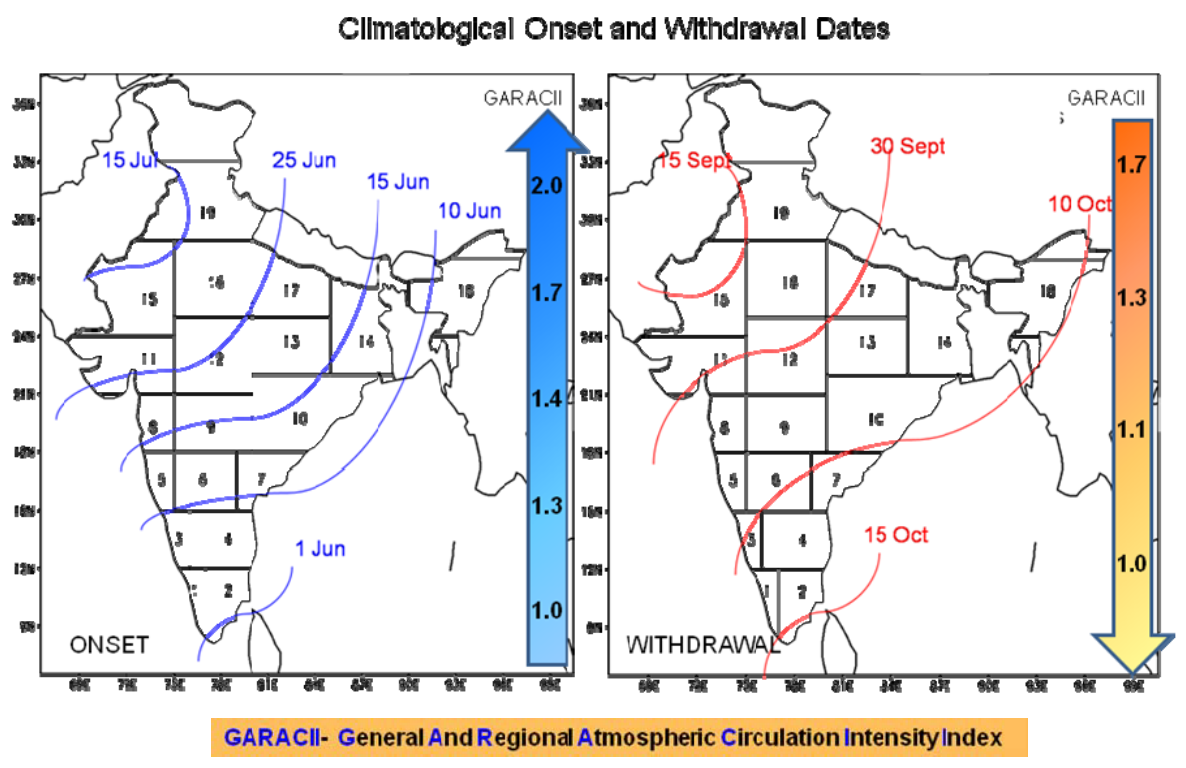
\includegraphics[width=0.6\textwidth]{./99_appendix/img/singh_subregions.png}
  \caption{Regular monsoon onset and withdrawal dates for the 19 subregions of the Indian subcontinent as depicted in \citet{Singh.2009}.}
  \label{fig:singh_subregions}
\end{figure}

\paragraph{Prediction of monsoon withdrawal}
While we have focused on predicting the monsoon onset, the withdrawal of monsoon is of similarly high importance to the Indian population, as it marks the transition from the rainy season to the winter months. Basing on our final model architecture, the withdrawal dates of the ISM could be predicted without necessitating any large changes. Using data for the monsoon season as extracted from ERA-Interim and onset dates from the IMD and \citet{Singh.2009}, a well-tuned model should be able to predict monsoon withdrawal with reasonable accuracy.
